\documentclass[12pt,a4paper]{article}

%\setlength{\textwidth}{7.0in}
\setlength{\topmargin}{-.80in}
%\setlength{\leftmargin}{0.0in}
\setlength{\evensidemargin}{-.40in}
\setlength{\oddsidemargin}{-.23in}
\setlength{\textheight}{9.95in}
\setlength{\textwidth}{7.00in}
\setlength{\marginparwidth}{-.50in}

%\setlength{\textheight}{8in}

\usepackage{url}
\usepackage{amsmath}
\usepackage{amsfonts}
%\usepackage{lastpage}
\usepackage{xspace}
\usepackage{paralist}
%\usepackage{setspace}
%\doublespacing
\usepackage{wrapfig}
\usepackage{graphicx}
%\usepackage{setspace,natbib}
%\usepackage[small,compact]{titlesec}
%\usepackage[small]{titlesec}
\usepackage{multicol}
\usepackage{xcolor}
\usepackage{verbatim}
\usepackage{xspace}

\newcommand{\lap}{\nabla}
\newcommand{\hf}{\frac{1}{2}}
\newcommand{\shf}{\frac{1}{2}}
\newcommand{\pdiff}[2]{\frac{\partial #1}{\partial #2}}

\definecolor{darkred}{rgb}{.5,0,0}
\definecolor{darkblue}{rgb}{0,0,0.3}
\definecolor{grey}{rgb}{0.6,0.6,0.6}
\usepackage[colorlinks=true,citecolor=darkblue,urlcolor=blue,linkcolor=darkred]{hyperref}
\usepackage{url}
\usepackage{fancyvrb}

\usepackage{accsupp}
%\renewcommand{\thelinenumber}{% Line number printing mechanism
%  \BeginAccSupp{ActualText={}}\arabic{linenumber}\EndAccSupp{}%
%}
\newcommand{\prompt}{%
  \BeginAccSupp{ActualText={}}\textcolor{grey}{\texttt{>>}}\EndAccSupp{}%
}


\renewcommand{\FancyVerbFormatLine}[1]{\prompt~#1}
\DefineVerbatimEnvironment{ml}{Verbatim}{gobble=2,samepage=true,xleftmargin=6ex, commandchars=\\\{\}
}


\newcommand{\Real}{\mathbb{R}}
\newcommand{\cp}{\textrm{cp}}
\newcommand{\grad}{\nabla}


%\setlength{\parskip}{1in}
%\addtolength{\parskip}{1in}
\addtolength{\parskip}{.2\baselineskip}

%\newlength{\saveparindent}
%\setlength{\saveparindent}{\parindent}
%\newlength{\saveparskip}
%\setlength{\parskip}{\saveparskip}
%\setlength{\parindent}{0pt}
%\setlength{\parskip}{.2\baselineskip}

\renewcommand{\figurename}{Fig.}


% Different font in captions
\newcommand{\captionfonts}{\small}

\makeatletter  % Allow the use of @ in command names
\long\def\@makecaption#1#2{%
  \vskip\abovecaptionskip
  \sbox\@tempboxa{{\captionfonts #1: #2}}%
  \ifdim \wd\@tempboxa >\hsize
    {\captionfonts #1: #2\par}
  \else
    \hbox to\hsize{\hfil\box\@tempboxa\hfil}%
  \fi
  \vskip\belowcaptionskip}
\makeatother   % Cancel the effect of \makeatletter

%\DefineShortVerb{\|}

%\usepackage{bibspacing}
%\setlength{\bibspacing}{\baselineskip}
%\setlength{\bibspacing}{2ex}

\newcommand{\Matlab}{\textsc{Matlab}\xspace}
\newcommand{\matlab}{\Matlab}


\begin{document}

\pagestyle{empty}

\begin{center}
  \begin{Large}
    \bf Image Processing Project for CBL Summer School
  \end{Large}

\end{center}


%\maketitle

%\section*{blah}

%\bigskip

\paragraph{Perona--Malik Image denoising} 
%On a previous homework we looked at non-constant diffusion.
In the lectures, we looked at spatially varying diffusion, where the diffusion coefficient varied with $x$ and $y$: now we go fully nonlinear with an application in image processing.

%\begin{aligned}
\begin{wrapfigure}{r}{0.38\textwidth}
  %\begin{center}
  %\vspace{-0.25in}%
  \hfill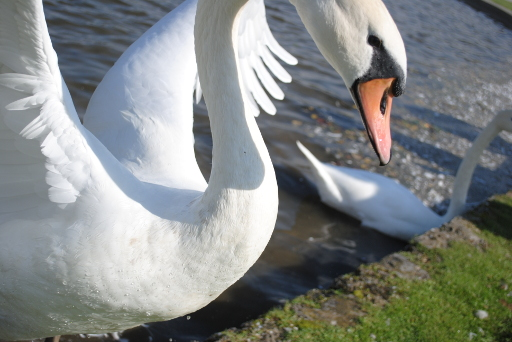
\includegraphics[width=0.35\textwidth]{swan-512}\\

  \vspace*{-3.5ex}

  {\scriptsize \hspace*{2em}
      Photograph by Harry Biddle}

  %\end{center}
  %\caption{Photograph by Harry Biddle (hb@dneg.com)}
  \label{fig:bunny}
\end{wrapfigure}
% \begin{center}
%   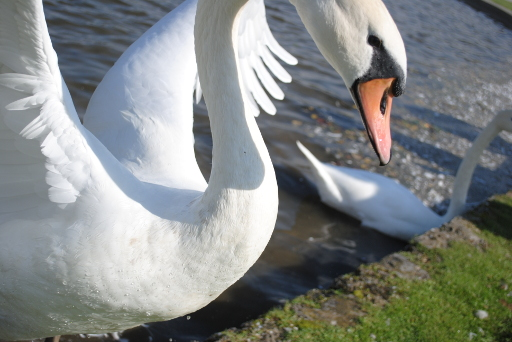
\includegraphics[width=0.35\textwidth]{swan-512}\\
%   \vspace*{-1.3ex}%
%   {\scriptsize %\hspace*{4em}
%     Photograph by Harry Biddle (hb@dneg.com)}
% \end{center}

First try regular diffusion (the heat equation in 2D). You can use the 
\url{diffusion1.m} and \url{isotropic_diffusion.m} codes from the github 
repository. This is Gaussian blurring.  It should get rid of the noise but it will also
blur all the detail in the image and in particular the \emph{edges}.
% TODO: fix this in a later year

The Perona--Malik equation is a
modification of Gaussian diffusion that employs edge preservation by
varying the diffusion coefficient across the image dependent on the image gradient $\nabla u$, penalising it at edges (i.e. where $\nabla u$ is large).
%and structures that should be preserved in the image.
The general equation is
$$u_t = \nabla \cdot \big( g(|\nabla u|) \nabla u \big),
\qquad \text{where} \qquad
g(s) = \frac{1}{1+\frac{s^2}{\lambda^2}}$$
is an edge detection function with a tunable parameter $\lambda$ that
controls the sensitivity of the equation to visual edges.  It gives a
threshold to separate noise from edges.

%TODO: give them some code.


The two-dimensional Cartesian form of the Perona--Malik equation is
\begin{equation*}
  \pdiff{u}{t} =
  \pdiff{}{x} \Big[ g\Big(\!\sqrt{u_x^2+u_y^2}\Big) \,u_x \Big] + \\
  \pdiff{}{y} \Big[ g\Big(\!\sqrt{u_x^2+u_y^2}\Big) \,u_y \Big].
\end{equation*}
Following the lectures on spatially varying diffusion, this can be discretized with finite differences and forward Euler
\begin{subequations}
\begin{align}
    u^{n+1}_{i,j} = u^n_{i,j} + \Delta t \bigg[
    \frac{g^n_{i+\shf,j} \, D^x_+ u^n_{i,j} - g^n_{i-\shf,j} \, D^x_- u^n_{i,j}}{\Delta x} \, + 
    \frac{g^n_{i,j+\shf} \, D^y_+ u^n_{i,j} - g^n_{i,j-\shf} \, D^y_- u^n_{i,j}}{\Delta x}
    \bigg]. \label{eq:gdiv}
\end{align}
Here $D^{\alpha}_+$ and $D^{\alpha}_-$ indicate forward and
backward finite differences, in the direction indicated by the
superscript $\alpha$, on a grid spacing of $\Delta x$.
The expressions involving $g$ between grid points are calculated as
the average of the values at the two neighbouring grid points, e.g.,
%\todo{we first construct a values of $g$ at the centers of computational cells, and
%then take the approximations at the boundary to be the average across the two cells that share it. Namely, we take}
\begin{equation}\label{eq:gbc}
  g^n_{i+\shf,j} = \tfrac{1}{2}( g^n_{i+1,j} + g^n_{i,j} ),
  \qquad
  g^n_{i-\shf,j} = \tfrac{1}{2}( g^n_{i-1,j} + g^n_{i,j} ),
\end{equation}
where the nodal $g^n_{i,j}$ are computed using central finite
differences
% $D^{\alpha}_c$ applied to $g(|\nabla u|)$
\begin{equation}\label{eq:gnodes}
  g^n_{i,j} = g\!\left(\!\sqrt{
        (D^x_c u^n_{ij})^2 +
        (D^y_c u^n_{ij})^2} \right)\!.
\end{equation}
\end{subequations}


Use the code from the github repository which loads the image and adds
noise.  Write a code to perform Perona--Malik denoising, using zero-Neumann boundary conditions for $u$. How does this set the boundary conditions for $g(|\nabla u|)$? Assuming you choose to make $\Delta x = 1$, then you might start with $\Delta t = 0.05$
and $\lambda = 1/100$. What happens to the diffusion near the edges?

Optional: try working with the full colour image.  One approach is to
work on each colour channel separately, although maybe R-G-B is not
the best basis.


\bibliographystyle{abbrv}
\bibliography{cbm}

\end{document}
